\section{Simulated multi-channel signal}
\label{sc:mysimulation}
To demonstrate the signal processing approach, this section generates simulated signals at resolutions ranging from 40cm down to 10cm. As already mentioned, the more the resolution decreases (i.e. improves) the greater the data capture, storage and signal processing requirements. The 12cm and 10cm modes required a significant amount of processing power, time and Random Access Memory (RAM). These modes were simulated by using the Vienna Super computing Cluster (VSC) for which the authors are deeply grateful. 
\par
The simulations, with parameters listed in \Tbref{tb:simulation}, were developed using the Python libraries Numba, Numpy, Scipy and Matplotlib. 
% \begin{table}[ht!]
% \begin{center}
%  \caption{Simulation parameters}
%  \label{tb:simulation}
%  \begin{tabular}{r|l|l|l|l|l|l}
%   mode & {\bf 40 cm} & {\bf 30 cm} & {\bf 25 cm} & {\bf 20 cm} & {\bf 12 cm} & {\bf 10 cm}\\\hline
%   $f_p$ (Hz) & $4500$ & $6428$ & $8181$ & $4500$ & $6428$ & $8181$\\\hline
%   $\antennaLengthEffective$ (m) & $4.0$ & $2.8$ & $2.2$ & $4.0$ & $2.8$ & $2.2$\\\hline
%   $\antennaLength$ (m) & $20.0$ & $19.6$ & $24.2$ & $20.0$ & $19.6$ & $24.2$\\\hline
%   $M+1$ & $5$ & $7$ & $11$ & $5$ & $7$ & $11$\\\hline
%   Swath (km) & $16.5$ & $7.5$ & $3$ & $16.5$ & $7.5$ & $3$\\\hline
%   $\carrier$ (GHz) & $9.65$ & $9.65$ & $9.65$ & $9.65$ & $9.65$ & $9.65$\\\hline
%   $B$ (MHz) & 374.74 & 499.65 & 599.58 & 749.48 & 1249.14 & 1498.96
%  \end{tabular}
%  \end{center}
% \end{table}
\begin{table}[ht!]
\begin{center}
 \caption{Simulation parameters}
 \label{tb:simulation}
 \begin{tabular}{r|l|l|l|l|l|l|l}
  {} & {\bf $f_p$} & {\bf $\antennaLength$} & {\bf $\antennaLengthEffective$} & {\bf $M+1$} & {Swath} & {\bf $\carrier$} & {\bf $B$}\\
 {mode}      & {Hz}    & m    & m   &   & km   & GHz  & MHz\\\hline
 {\bf 40 cm} & 4500.00 & 20.0 & 4.0 & 5 & 16.5 & 9.65 & 374.74\\\hline
 {\bf 30 cm} & 5000.00 & 21.4 & 3.6 & 6 & 13.5 & 9.65 & 499.65\\\hline
 {\bf 25 cm} & 5142.86 & 24.4 & 3.5 & 7 & 12.7 & 9.65 & 599.58\\\hline
 {\bf 20 cm} & 6428.57 & 19.6 & 2.8 & 7 & 7.5  & 9.65 & 749.48\\\hline
 {\bf 12 cm} & 7500.00 & 24.0 & 2.4 & 10 & 4.5 & 9.65 & 1249.14\\\hline
 {\bf 10 cm} & 8181.82 & 24.2 & 2.2 & 11 & 3.0 & 9.65 & 1498.96\\\hline
 \end{tabular}
 \end{center}
\end{table}
In the table, the swath width has been computed in the slant-range. The projection onto the ground yields, as a function of the incidence angle, a longer ground swath. The estimate for the slant-range swath is computed as
\begin{equation}
 \text{Swath}(f_p; \tau_p) = \left(1/f_p - 2*\tau_p\right)*\frac{c}{2}\times 90\%
\end{equation}
where $\tau_p$ is the pulse duration which was, for the table, selected as $\tau_p=50\times10^{-6}$ s. A 10\% margin has also been incorporated.
\par
The satellite velocity chosen for the simulation is 7500 m/s. This means that the \gls{dpca} condition is not met for any of the simulations. All \gls{prf}s have been increased by a factor of 1.2 relative to the one that matches the \gls{dpca} condition.
\par
As outlined in \fgref{fg:simflow}, the simulator computes the back-folded signal for each of the desired channels of data, computes the processing filters, applies the filters to the back-folded data and presents the amplitude of the reconstructed signal in the Doppler domain.
\begin{figure}[ht!]
\begin{center}
 \resizebox{0.5\columnwidth}{!}{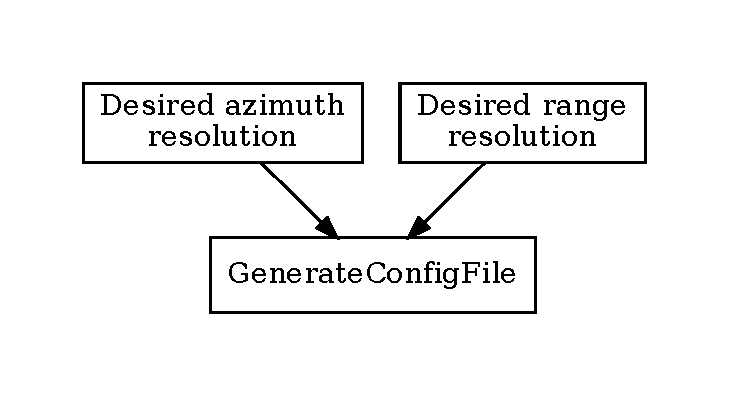
\includegraphics{sim.pdf}}
 \caption{Simulation of the SURE signal.}
 \label{fg:simflow}
 \end{center}
\end{figure}
\subsection{Generation of the raw signals}
All simulations for this paper utilize a phased array with elements of width 0.04m which are ideally spaced 0.04m apart, see \fgref{fg:fivechansubaperture}. For instance, the phased array used for the 40cm mode is described by the XML snippet shown in Listing \ref{lst:array}.
\lstset{language=XML}
\begin{lstlisting}[caption={Phased Array configuration}, label={lst:array}]
<instrument>
  <antennaArray>
    <carrierFrequency unit="Hz">9.650e9</carrierFrequency>
    <azimuthPositions unit="m">-9.980000 -9.940000 -9.900000 ...
    ... 9.900000 9.940000 9.980000</azimuthPositions>
    <azimuthElementLengths unit="m">0.040000 0.040000 0.040000 ...
    ... 0.040000 0.040000 0.040000</azimuthElementLengths>
    <transmitPowers unit="dB">10.0 10.0 10.0 ...
    ... 10.0 10.0 10.0</transmitPowers>
    <systemTemperature unit="degrees" system="Kelvin">297</systemTemperature>
    <systemLosses unit="dB">-5.3</systemLosses>
  </antennaArray>
</instrument>
\end{lstlisting}
The azimuthPositions XML field defines the position of each T/R module in the azimuth direction while the azimuthElementLength defines the width of each element.
\par
The various azimuth look directions are defined according to the angular width of each beam (which depends upon the length of the subaperture) and the span of angles required to achieve a particular azimuth resolution. In this simulation all beams are created with the same angular width. As well, the subaperture phase-centre positions are generated to be evenly spaced in the azimuth direction.
\begin{figure}[h!]
\begin{center}
 \resizebox{0.7\columnwidth}{!}{\input{subarray.pdf_tex}}
 \caption{Schematic of 5 subapertures for the 40 cm mode.}
 \label{fg:fivechansubaperture}
 \end{center}
\end{figure}
\par
As illustrated in \fgref{fg:fivechansubaperture}, the simulation generates a data array for each subaperture/beam combination. The parameters for for each subaperture/beam combination are also read from the configuration file as illustrated in Listing \ref{lst:configuration}. For each of these combinations, the configuration file defines an XML element called radarConfiguration which has a channel attribute given by ``channel$m$-$n$'', where $m$ corresponds to the subaperture while $n$ corresponds to the beam. The subaperture is defined using magnitude weights for each phased-array element on both transmit and receive. The set of wieghts used on transmit may be different from those used on receive. 
\par
The beam directions are controlled by using true time-delays on both transmit and receive (although they are set to the same values in this simulation so that the transmit and receive beams are pointing in the same direction). Of course, a true time-delay approach rather than a phase-steered approach is required as we are considering a wideband system rather than a narrowband system.
\begin{lstlisting}[caption={Channel/Beam configuration}, label={lst:configuration}]
<radarConfiguration channel="channel0-0">
  <transmitConfiguration>
    <polarization>H</polarization>
    <u0 unit="radians">1.553329e-02</u0>
    <magnitude unit="natural">0 0 0 ... 1 1 1 ... 0 0 0</magnitude>
    <truedelay unit="ns">0.517098 0.515026 0.512953 ...</truedelay>
  </transmitConfiguration>
  <receiveConfiguration>
    <polarization>H</polarization>
    <u0 unit="radians">1.553329e-02</u0>
    <magnitude unit="natural">1 1 1 ... 0 0 0 ... 0 0 0</magnitude>
    <truedelay unit="ns">0.517098 0.515026 0.512953 ...</truedelay>
  </receiveConfiguration>
</radarConfiguration>
\end{lstlisting}
A data file for each subaperture/beam combination is created with the data stored in the undersampled azimuth-wavenumber, range-time domain. The number of samples in each of the subaperture/beam combinations is sufficient in the range direction to cover all range-cell migration and sufficient in the azimuth direction to capture all angles covered by every beam. Since the number of beams equals the number of channels, the total number of channels created is $\numberChannels = (\channelM+1)^2$.
\par
Note that in this simulation, the computed signals have no across-track baseline.
\subsection{Multi-channel processing}
Multi-channel processing for this simulation occurs in the azimuth-wavenumber, range-time domain. This step computes a processing filter that attempts to create a signal over an azimuth frequency range given by $\kparmPRF*(\numberChannels + 4)$; that is, when the average antenna pattern of \eqref{eq:averagePattern} is applied, there should some wavenumber domain zero-padding applied to the computed signal.
\par
Since the theory shows that the multi-channel processing filter is range independent, only a single processing filter is computed and applied across all ranges. \Fgref{fg:reconstructed} illustrates the multi-channel processed signal. In the figure, one sees that the response in the Doppler domain shows the desired response as a function of $\kparm$, with each local maximum in this region highlighting the response from each sub-beam.
\begin{figure}[ht!]
\begin{subfigure}{0.5\textwidth}
\begin{center}
 \resizebox{\columnwidth}{!}{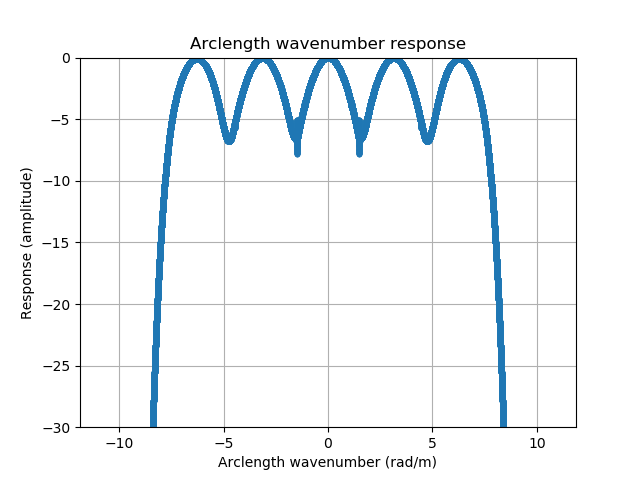
\includegraphics{simulation/40cm/simulation_plots/wk_doppler_response_amplitude.png}}
 \caption{40 cm mode.}
 \label{fg:40cmreconstructed}
 \end{center}
\end{subfigure}
\begin{subfigure}{0.5\textwidth}
\begin{center}
 \resizebox{\columnwidth}{!}{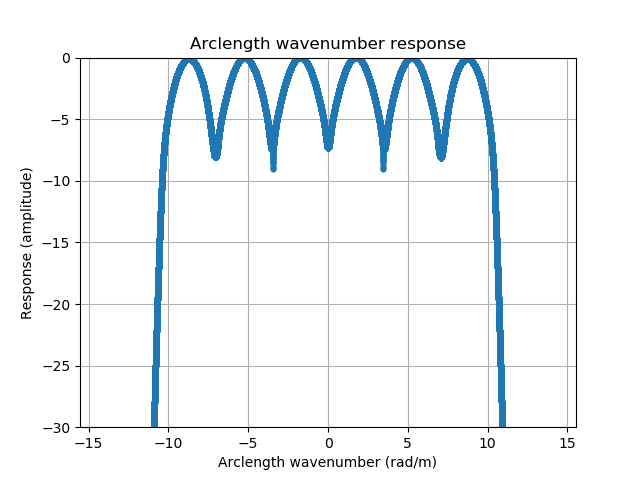
\includegraphics{simulation/30cm/simulation_plots/wk_doppler_response_amplitude.png}}
 \caption{30 cm mode.}
 \label{fg:30cmreconstructed}
 \end{center}
\end{subfigure}
\begin{subfigure}{0.5\textwidth}
\begin{center}
 \resizebox{\columnwidth}{!}{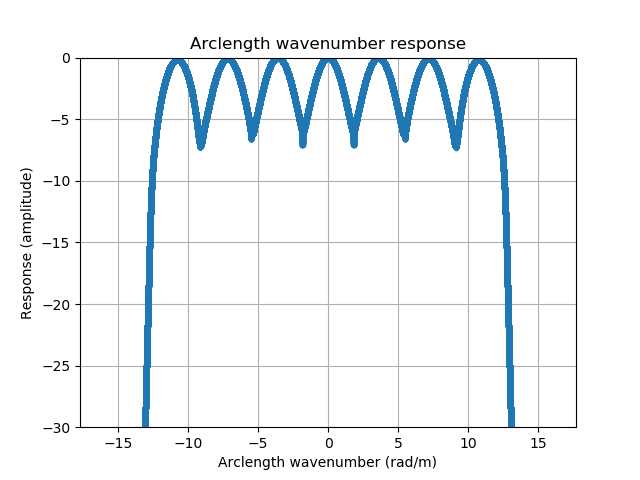
\includegraphics{simulation/25cm/simulation_plots/wk_doppler_response_amplitude.png}}
 \caption{25 cm mode.}
 \label{fg:25cmreconstructed}
 \end{center}
\end{subfigure}
\begin{subfigure}{0.5\textwidth}
\begin{center}
 \resizebox{\columnwidth}{!}{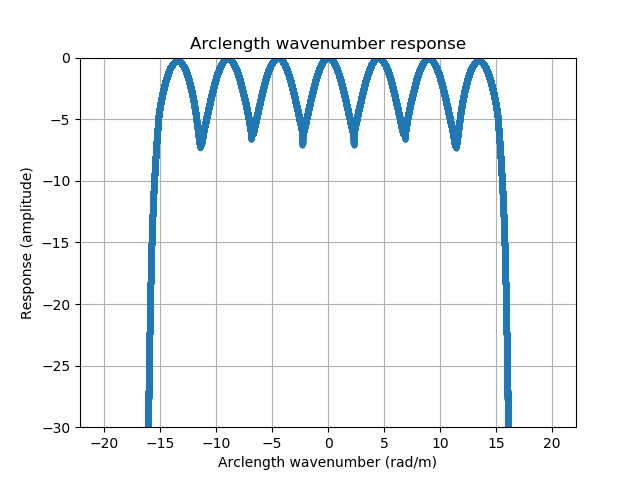
\includegraphics{simulation/20cm/simulation_plots/wk_doppler_response_amplitude.png}}
 \caption{20 cm mode.}
 \label{fg:20cmreconstructed}
 \end{center}
\end{subfigure}
\begin{subfigure}{0.5\textwidth}
\begin{center}
 \resizebox{\columnwidth}{!}{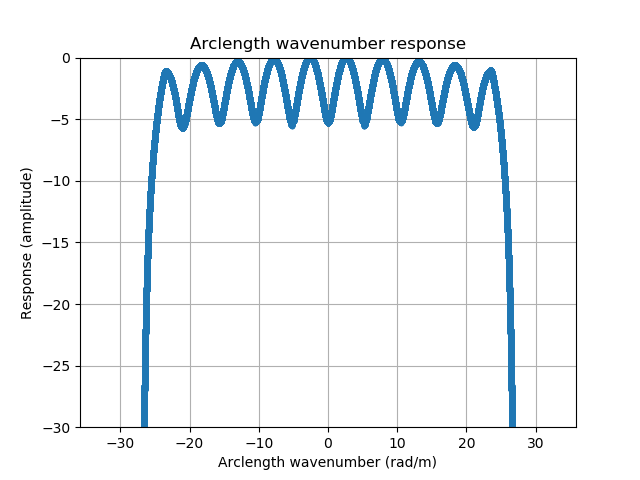
\includegraphics{simulation/12cm/simulation_plots_full/wk_doppler_response_amplitude.png}}
 \caption{12 cm mode.}
 \label{fg:12cmreconstructed}
 \end{center}
\end{subfigure}
\begin{subfigure}{0.5\textwidth}
\begin{center}
 \resizebox{\columnwidth}{!}{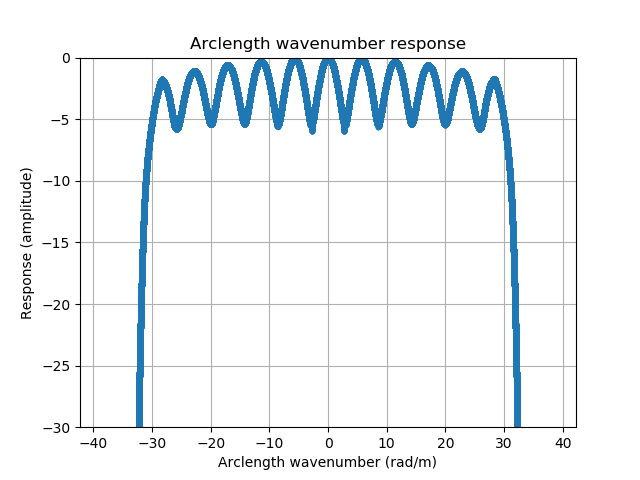
\includegraphics{simulation/10cm/simulation_plots_phase_corrected/wk_doppler_response_amplitude.png}}
 \caption{10 cm mode.}
 \label{fg:10cmreconstructed}
 \end{center}
\end{subfigure}
\caption{Reconstructed signals in azimuth wavenumber domain.}
\label{fg:reconstructed}
\end{figure}
\clearpage
\subsection{Azimuth compression}
The simulator then azimuth compresses multi-channel reconstructed signal with the generalized Stolz interpolation algorithm outlined in \scref{sc:modifiedStolz}. \Fgref{fg:PSFAll} illustrates the produced Point Spread Functions (PSF) for all modes. In these plots, the residual phase correction of \scref{sc:phaseCompensation} has not been applied.
\begin{figure}[ht!]
\begin{subfigure}{0.5\textwidth}
\begin{center}
 \resizebox{\columnwidth}{!}{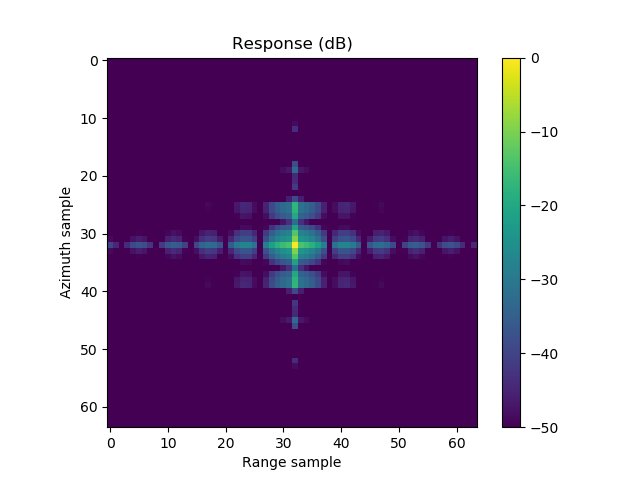
\includegraphics{simulation/40cm/simulation_plots/wk_response_32x32.png}}
 \caption{40 cm mode.}
 \label{fg:40cmPSF}
 \end{center}
\end{subfigure}
\begin{subfigure}{0.5\textwidth}
\begin{center}
 \resizebox{\columnwidth}{!}{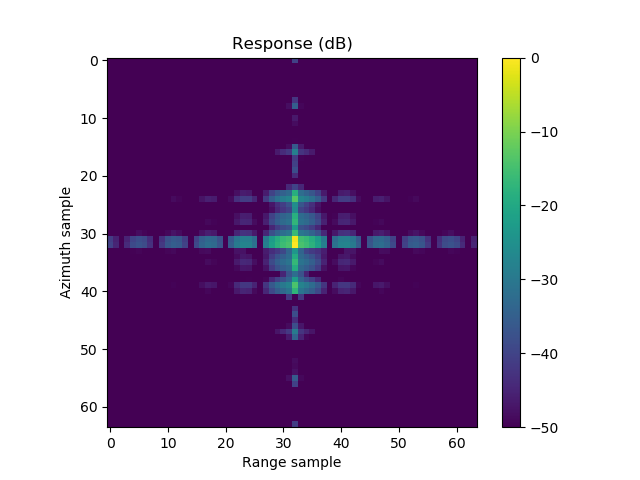
\includegraphics{simulation/30cm/simulation_plots/wk_response_32x32.png}}
 \caption{30 cm mode.}
 \label{fg:30cmPSF}
 \end{center}
\end{subfigure}
\begin{subfigure}{0.5\textwidth}
\begin{center}
 \resizebox{\columnwidth}{!}{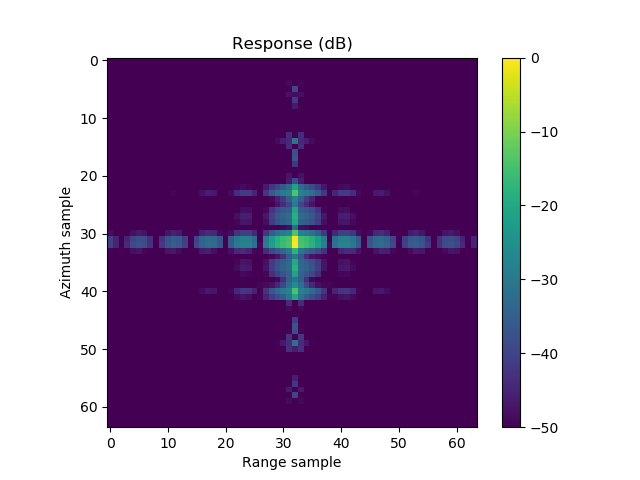
\includegraphics{simulation/25cm/simulation_plots/wk_response_32x32.png}}
 \caption{25 cm mode.}
 \label{fg:25cmPSF}
 \end{center}
\end{subfigure}
\begin{subfigure}{0.5\textwidth}
\begin{center}
 \resizebox{\columnwidth}{!}{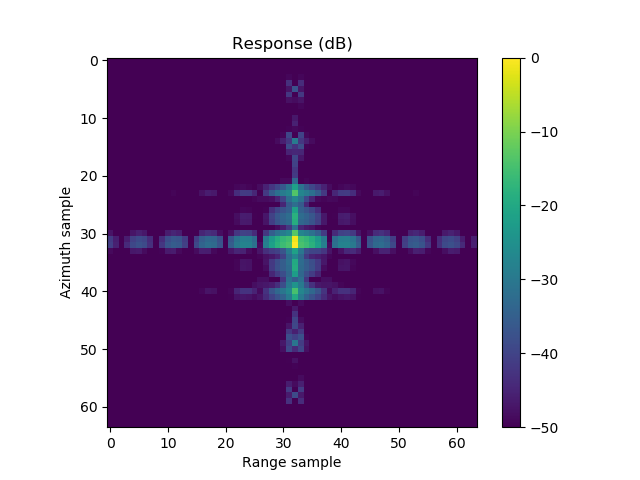
\includegraphics{simulation/20cm/simulation_plots/wk_response_32x32.png}}
 \caption{20 cm mode.}
 \label{fg:20cmPSF}
 \end{center}
\end{subfigure}
\begin{subfigure}{0.5\textwidth}
\begin{center}
 \resizebox{\columnwidth}{!}{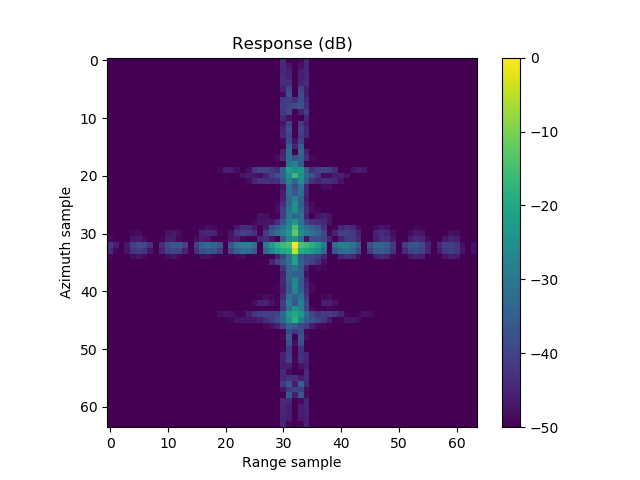
\includegraphics{simulation/12cm/simulation_plots_full/wk_response_32x32.png}}
 \caption{12 cm mode.}
 \label{fg:12cmPSF}
 \end{center}
\end{subfigure}
\begin{subfigure}{0.5\textwidth}
\begin{center}
 \resizebox{\columnwidth}{!}{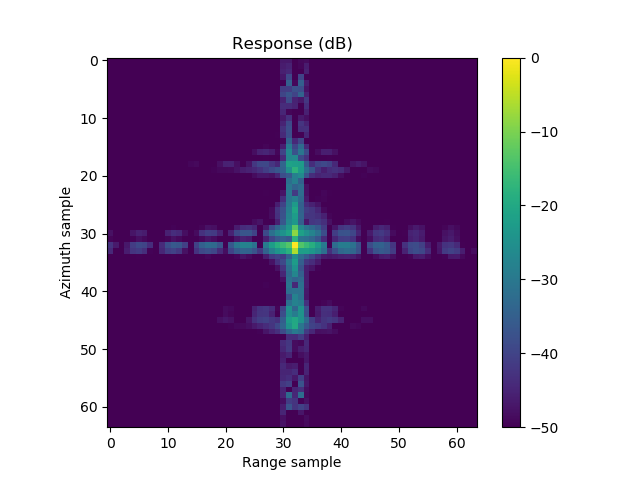
\includegraphics{simulation/10cm/simulation_plots/wk_response_32x32.png}}
 \caption{10 cm mode.}
 \label{fg:10cmPSF}
 \end{center}
\end{subfigure}
\caption{Processed signal Point Spread Response.}
\label{fg:PSFAll}
\end{figure}
\clearpage
\subsubsection{Residual phase correction}
As the resolution increases, it becomes more important to compensate for the residual phase difference that arises from the discrepancy between the differential geometry approximation to the orbit and the true satellite orbit. If examined closely, \fgref{fg:10cmPSF} shows an azimuth imbalance in the the PSF for the 10cm mode (this can also be seen in the 12cm mode and in the 20 cm mode). This imbalance is made clearer in the cross-section plot of \fgref{fg:azimuthCross10Unbalanced}.
\begin{figure}[ht!]
\begin{center}
 \resizebox{\columnwidth}{!}{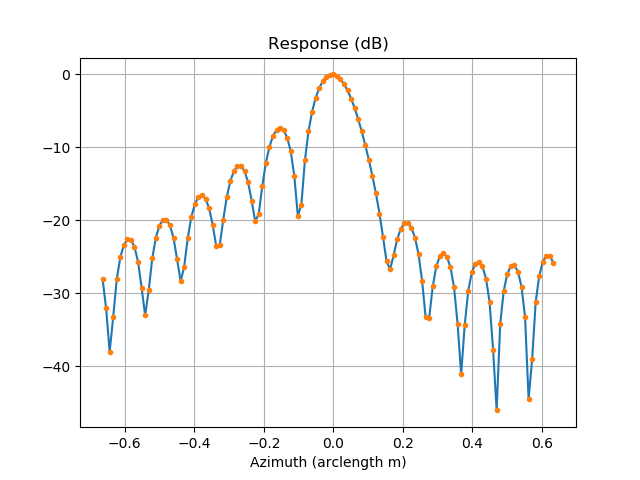
\includegraphics{simulation/10cm/simulation_plots/wk_response_s_os_8.png}}
 \caption{Azimuth cross-section of 10cm mode without residual phase correction.}
 \label{fg:azimuthCross10Unbalanced}
 \end{center}
\end{figure}
After compensating for the residual phase using the computed phase compensation described in \scref{sc:phaseCompensation}, one obtains the more desirable point spread function illustrated in \fgref{fg:10cmPSFBalanced} along with its azimuth cross-section illustrated in \fgref{fg:azimuthCross10}.
\begin{figure}[ht!]
\begin{center}
 \resizebox{\columnwidth}{!}{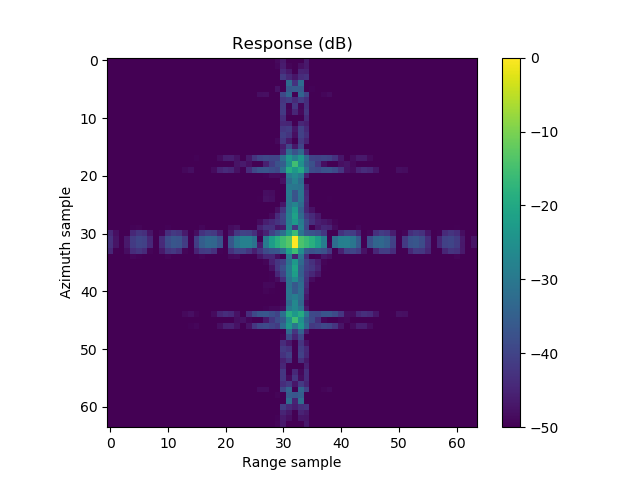
\includegraphics{simulation/10cm/simulation_plots_phase_corrected/wk_response_32x32.png}}
 \caption{Point Spread Function of 10cm mode after phase compensation.}
 \label{fg:10cmPSFBalanced}
 \end{center}
\end{figure}
\begin{figure}[ht!]
\begin{center}
 \resizebox{\columnwidth}{!}{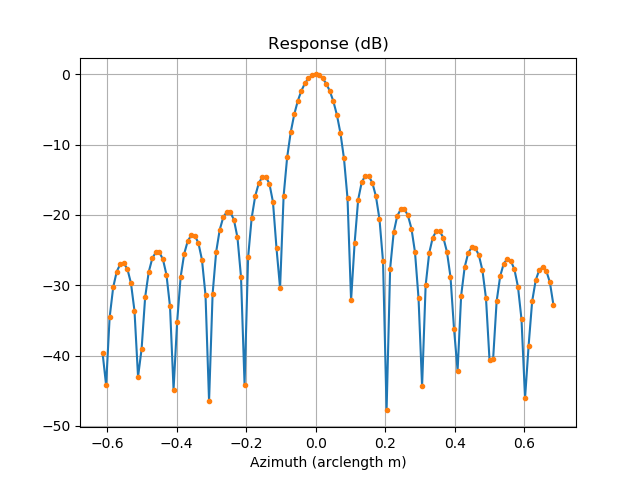
\includegraphics{simulation/10cm/simulation_plots_phase_corrected/wk_response_s_os_8.png}}
 \caption{Azimuth cross-section of 10cm mode after residual phase correction.}
 \label{fg:azimuthCross10}
 \end{center}
\end{figure}
The plot clearly illustrates a 3dB resolution of better than 10cm. Further, in the generation of sidelobes at this zoom level, the peak sidelobe level is at around -14.5dB from the peak.
\par
Over the wider range of azimuth values illustrated in \fgref{fg:azimuthCross10wide}, one observes a different generation of sidelobes. The peak of these second-level sidelobes manifests at around -18dB. A suitable weighting on the Doppler response of \fgref{fg:10cmPSF} can suppress these second-level sidelobes at the expense of resolution.
\begin{figure}[ht!]
\begin{center}
 \resizebox{\columnwidth}{!}{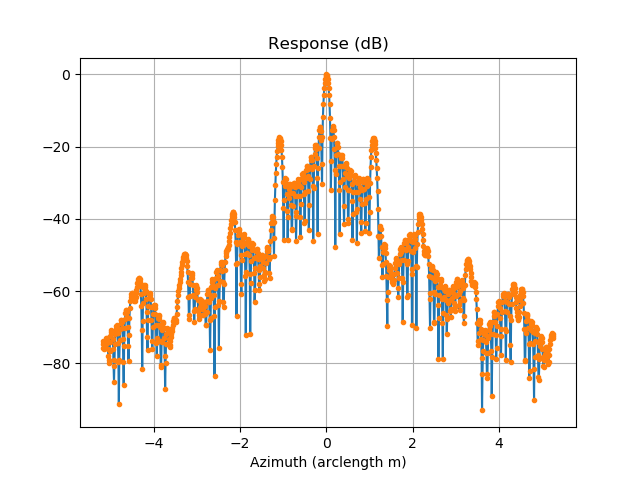
\includegraphics{simulation/10cm/simulation_plots_phase_corrected/wk_response_s_os_64.png}}
 \caption{Azimuth cross-section of 10cm mode after residual phase correction.}
 \label{fg:azimuthCross10wide}
 \end{center}
\end{figure}
% shown in \fgref{fg:psf}. This figure illustrates that the system achieves the desired resolution with the response width less than 0.1 m at the -5 dB level. While the figure also shows a second set of sidelobes at -15 dB, it is assumed that these can be reduced by an appropriate choice of weighting on the antenna patterns. 
% \begin{figure}[ht!]
% \begin{center}
%  \resizebox{\columnwidth}{!}{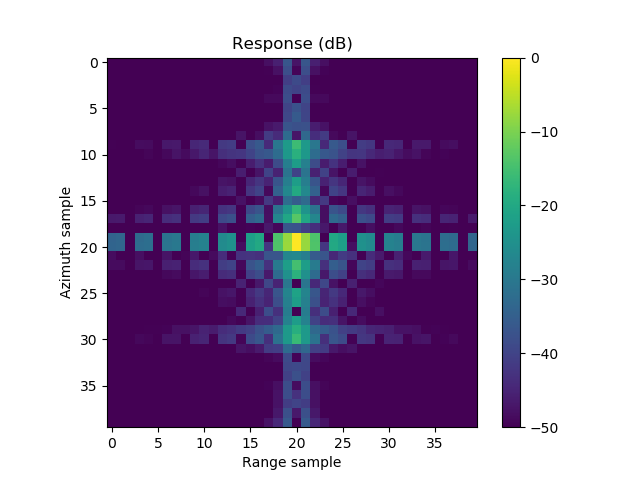
\includegraphics{simulation/Figure_11.png}}
%  \caption{Point Spread Function using the described processing method.}
%  \label{fg:psf}
%  \end{center}
% \end{figure}
% \begin{figure}[ht!]
% \begin{center}
%  \resizebox{\columnwidth}{!}{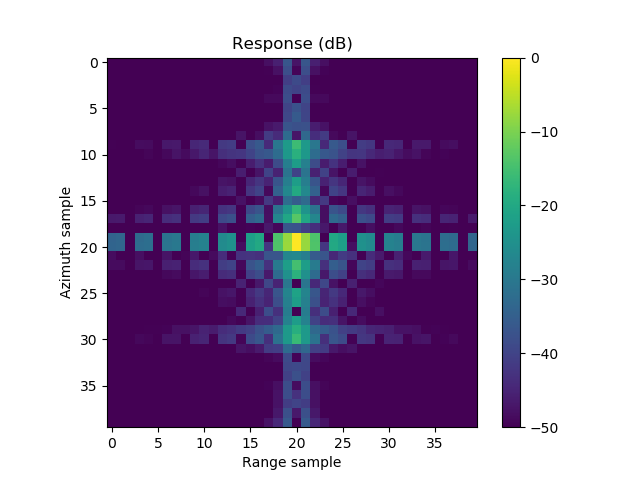
\includegraphics{simulation/Figure_11.png}}
%  \caption{Point Spread Function using the described processing method.}
%  \label{fg:psf1}
%  \end{center}
% \end{figure}
% \begin{figure}[ht!]
% \begin{center}
%  \resizebox{\columnwidth}{!}{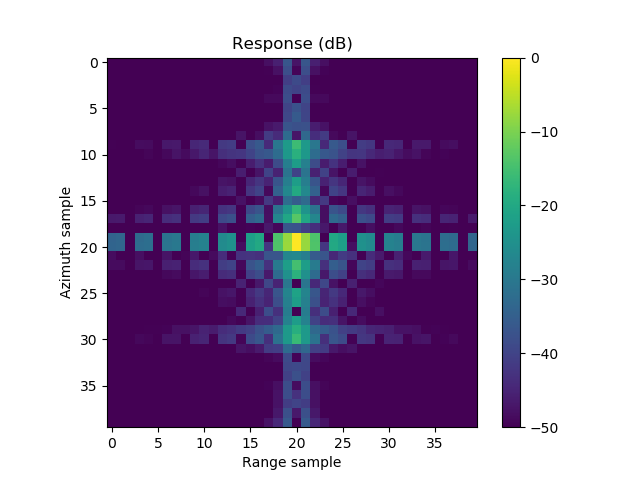
\includegraphics{simulation/Figure_11.png}}
%  \caption{Point Spread Function using the described processing method.}
%  \label{fg:psf2}
%  \end{center}
% \end{figure}
\subsubsection{Signal-to-noise ratio}
The PRFs selected for all simulations differ from the ``ideal'' \gls{dpca} \gls{prf} thus potentially adversely affecting the \gls{snr}. As a measure of the radiometrical resolution, the \gls{nesz} is computed for all modes. 
Based upon parameters in the simulation configuration file, the radar equation, \cite{Skolnik}, is used to generate a estimate of the simulated \gls{snr}. 
\par
Assuming ideal antenna elements, each with area $D_aD_e$, where $D_a$ and $D_e$ are the azimuth and elevation lengths of the antenna, then the gain of each element as a function of directional cosine $u$ in the azimuth direction and $v$ in the elevation direction may be represented as
\begin{equation}
 G_{T_x}(u,v) = G_{R_x}(u,v) = \frac{4\pi D_aD_e}{\lambda_0^2}\text{sinc}^2\left(\frac{uD_a}{\lambda_0}\right)\text{sinc}^2\left(\frac{vD_e}{\lambda_0}\right).
 \label{eq:gainPattern}
\end{equation}
This expression is such that
\begin{equation}
 \int_{-1}^1G_{T_x}(u,v)\d{u}\d{v}=4\pi,
\end{equation}
which simply means that power is preserved; however, rather than the power being evenly distributed around a sphere, it is directed, preferentially, in the direction $u=v=0$.
\par
If $P_{T_x}$ is the transmit power of each transmit element, then the true-time-delay beamforming operation (consisting of $N_{T_x}$ elements) delivers a total of power of $P_{\text{total}} = P_{T_x}N_{T_x}$, and the received \gls{snr} can be expressed as
\begin{equation}
 \frac{P_{\text{total}}G_{T_x}(u,v)A_{R_x}}{(4\pi R^2)^2Lk_BTB}\crossSection
\end{equation}
where $A_{R_x}=N_{R_x}A_e$ is the effective receive area and $A_e=D_aD_e\alpha$. Also, $k_B$ is Boltzmann's constant. Here, $\alpha<1$ accounts for the ``effective'' antenna area of each T/R module. Finally, $\crossSection$ is the backscatter cross-section. If one considers only the maximum gain (i.e. the maximum of \eqref{eq:gainPattern}), the above becomes
\begin{equation}
 \frac{P_{\text{total}}N_{R_x}A_e}{(4\pi R^2)^2Lk_BTB}\frac{4\pi N_{T_x}A_e}{\lambda_0^2}\crossSection
\end{equation}
where $A_{T_x}=N_{T_x}A_e$ is the effective area of the transmit antenna. The pulse compression gain is approximately $\tau_pB$ (where $\tau_p$ is the pulse duration), so, after pulse compression, one computes an \gls{snr} of
\begin{equation}
 \SNR_s = \frac{P_{\text{total}}N_{R_x}N_{T_x}A_e^2\tau_p}{4\pi R^4 Lk_BT\lambda_0^2}\crossSection
 \label{eq:pulseCompBeamFormedSNR}
\end{equation}
This is the \gls{snr} of each channel before multi-channel and SAR processing. The simulation sets the amplitude of return signal to $\sqrt{\SNR_s}$ with $\crossSection=1$ and generates an additive zero-mean complex circular Gaussian noise signal with unit variance. This noise signal is passed though the multi-channel and SAR processing steps with the same parameters used as for the signal thus simulating the processed noise. The NESZ is computed as the variance of this noise signal divided by the target signal (the maximum of the squared absolute value) yielding the results in \tbref{tb:nesz}. For all the modes simulated, the worst-case NESZ is -25 dB while the NESZ for the 10 cm mode is around -30 dB.
\begin{table}[ht!]
\begin{center}
 \caption{Computed NESZ}
 \label{tb:nesz}
 \begin{tabular}{r|l|l}
 {\bf Mode} & {\bf $f_p$} (Hz)& {\bf NESZ} (dB)\\\hline
 {\bf 40 cm} & 4500.00 & -30.9\\\hline
 {\bf 30 cm} & 5000.00 & -29.8\\\hline
 {\bf 25 cm} & 5142.86 & -29.7\\\hline
 {\bf 20 cm} & 6428.57 & -29.2\\\hline
 {\bf 12 cm} & 7500.00 & -25.5\\\hline
 {\bf 10 cm} & 8181.82 & -30.2\\\hline
 \end{tabular}
 \end{center}
\end{table}
\par
In summary, the simulation confirms the suitability of the proposed signal processing algorithm and also shows how the generated PSF contains extra sidelobes that most likely result from the different shape of the signal response in the Doppler domain. If these sidelobes are intolerable, they can possibly be removed by modifying the phased-array beam tables; however, this is a topic for further research. The simulation further shows that this approach to SAR imaging generates responses of very high resolution not only geometrically, but also with favourable NESZ characteristics.
\clearpage
%\section{Conclusion}
We propose a system for improved space-based SAR imaging, describing the design, which is based upon a phased-array and an appropriate switching network to allow digitisation of multiple receive channels, the configuration, which imposes a rapid electronic beam switching capability upon the design, and a suitable signal processing algorithm to compute the high resolution imagery. The proposed configuration permits measurement of a relatively large swath in a Stripmap-like mode, thereby offering, theoretically, unlimited azimuth extent. On the other hand, as demonstrated by the test example of 10cm azimuth resolution considered throughout the paper, the resolution of the imagery can be even better than the highest resolution spotlight imagery available from current commercial systems.
\par
Importantly, the state of current technology is sufficiently advanced to construct such a SAR system.
\par
As a final important consideration, we note that the design does not preclude the use of other traditional measurement modes such as Spotlight, TOPS or ScanSAR. Further, it provides the flexibility to implement other advanced modes such as HRWS and Ground Moving Target Indication.

